\chapter{Triển khai quy trình khai phá dữ liệu}\label{chapter_overview}

Phần này sinh viên viết các nội dung theo file hướng dẫn thực hiện bài tập lớn học phần.

\section{Mô tả pipeline}

(Hoặc Quy trình ứng dụng thuật toán để bảo mật và xác thực dữ liệu với nhóm đề tài bảo mật cơ sở dữ liệu)

\section{Phân tích mã nguồn và chức năng}
Nêu ngắn gọn súc tích cấu trúc repo, dẫn link repo Github. Không sa đà vào mô tả cụ thể đoạn code nào làm cái gì. Tuyệt đối KHÔNG copy code cho dài.

\section{Thiết kế thử nghiệm}


Các nội dung bên dưới hướng dẫn thực hiện chèn hình ảnh, công thức, bảng biểu, code vào báo cáo:

Hình \ref{icc_plot} minh họa chèn hình ảnh vào báo cáo.
 
\begin{center}
    \begin{figure}[h!]
    \begin{center}
     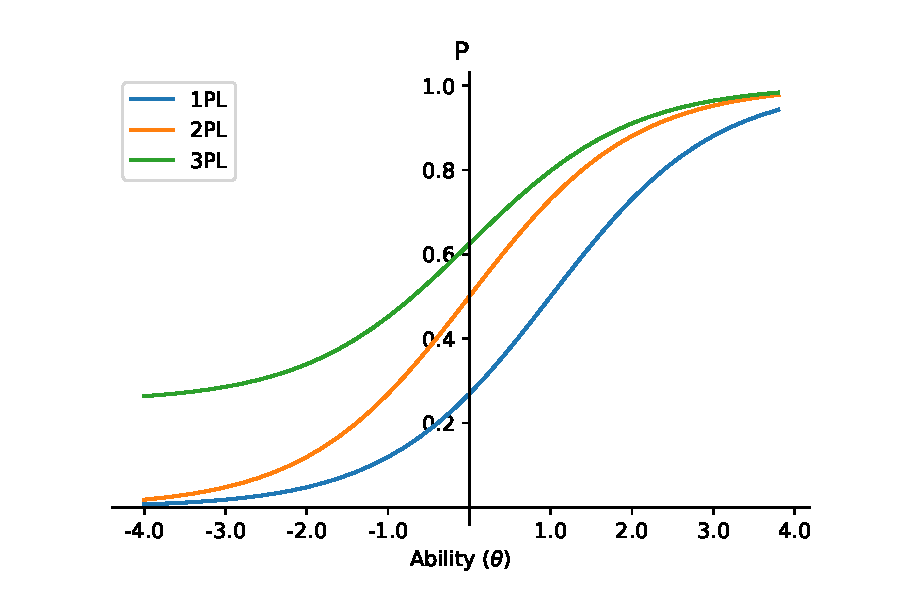
\includegraphics[scale=0.5]{figs/ICC_plots.pdf}
    \end{center}
    \caption{Một ví dụ về chèn hình ảnh.}
    \label{icc_plot}
    \end{figure}
\end{center}

Chèn bảng

\begin{center}
    \begin{table}
    \centering
    \caption{Ví dụ về tạo bảng trong \LaTeX. Tham khảo: \url{https://en.wikibooks.org/wiki/LaTeX/Tables}.}
        \begin{tabular}{ |l|l|l| }
        \hline
        \multicolumn{3}{ |c| }{Danh sách U23 Việt Nam tại Sea Games 31} \\
        \hline
        Thủ môn & GK & Nguyễn Văn Toản \\ \hline
        \multirow{4}{*}{Hậu vệ} & LB & Phan Tuấn Tài \\
         & DC & Bùi Hoàng Việt Anh \\
         & DC & Lê Văn Đô \\
         & RB & Lê Văn Xuân \\ \hline
        \multirow{3}{*}{Tiền vệ} & MC & Đỗ Hùng Dũng \\
         & MC & Nguyễn Hoàng Đức \\
         & MC & Dụng Quang Nho \\ \hline
        
        \multirow{2}{*}{Tiền đạo} & ST & Nhâm Mạnh Dũng \\
         & ST & Nguyễn Văn Tùng \\
         & FW & Nguyễn Tiến Linh \\
        \hline
        \end{tabular}
    
    \end{table}
\end{center}

Chèn công thức toán học

Công thức \ref{eq:InterTweetInteraction} thể hiện mức độ tương tác giữa hai tập $T_{j}^{P}$ và $T_{k}^{P}$.

\[
d(\mathbf{x},\mathbf{y})=\sqrt{\sum_{i=1}^{n}\bigl(x_i-y_i\bigr)^2}
\]


\begin{align}
S_{j,k}^{P}=\frac{\sum_{t_{m}^{P}\in T_{j}^{P}}\sum_{t_{n}^{P}\in T_{k}^{P}}r\left(t_{m}^{P},t_{n}^{P}\right)}{|T_{j}^{P}||T_{k}^{P}|}\label{eq:InterTweetInteraction}
\end{align}

Để soạn thảo các công thức toán học được dễ dàng hơn, có thể sử dụng một phần mềm hỗ trợ nhập công thức theo dạng What You See Is What You Mean (WYSIWYM), chẳng hạn như \href{https://www.lyx.org/}{LyX}, sau đó copy LaTeX code vào file .tex (xem Hình \ref{lyx_example}), sẽ được kết quả như Công thức \ref{eq:ErrorFunction}.

\begin{center}
    \begin{figure}[h!]
    \begin{center}
     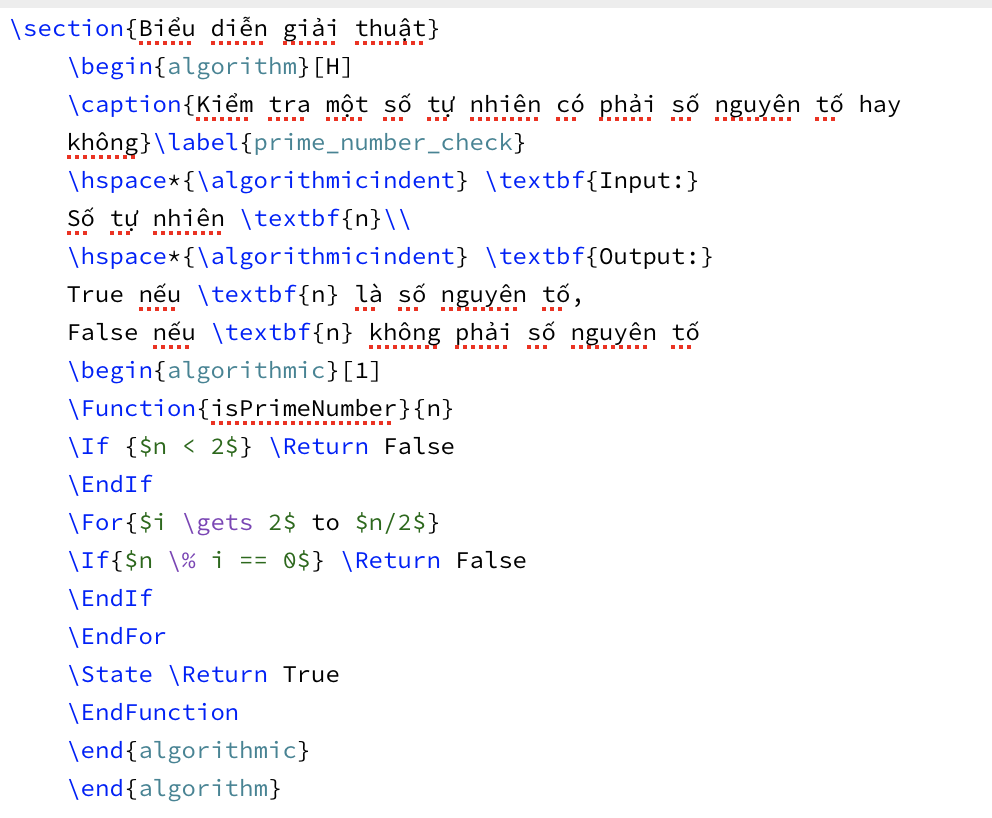
\includegraphics[scale=0.8]{figs/test.png}
    \end{center}
    \caption{Ví dụ cách soạn thảo công thức bằng LyX và copy sang file .tex.} 
    \label{lyx_example}
    \end{figure}
\end{center}

\begin{align}
E=\frac{1}{2}\sum_{i=1}^{n}(\hat{y}_{i}-y_{i})^{2}
\label{eq:ErrorFunction}
\end{align}


Chèn mã nguồn

Có thể sử dụng package minted để chèn mã nguồn có định dạng (syntax highlighted source code) vào báo cáo. Có hai lựa chọn:  chèn mã nguồn trực tiếp hoặc từ file có sẵn.

Chèn mã nguồn trực tiếp
\noindent\textbf{Ví dụ:}

\begin{minted}{C++}
#include<stdio.h>
int main()
{
	printf("Hello world!");
}
\end{minted}

Chèn mã nguồn từ file
\noindent\textbf{Cú pháp:} 
\begin{minted}{latex}
\inputminted{C++/Java/C#...}{path to source file}
\end{minted}
\noindent\textbf{Ví dụ:} Đoạn mã nguồn sau đây được chèn từ file \path{code/XulyFileText.cpp}

    \begin{algorithm}[H]
    \caption{Kiểm tra một số tự nhiên có phải số nguyên tố hay không}\label{prime_number_check}
    \hspace*{\algorithmicindent} \textbf{Input:} 
    Số tự nhiên \textbf{n}\\
    \hspace*{\algorithmicindent} \textbf{Output:} 
    True nếu \textbf{n} là số nguyên tố,
    False nếu \textbf{n} không phải số nguyên tố
    \begin{algorithmic}[1]
    \Function{isPrimeNumber}{n}
    \If {$n < 2$} \Return False
    \EndIf
    \For{$i \gets 2$ to $n/2$}
    \If{$n \% i == 0$} \Return False
    \EndIf
    \EndFor
    \State \Return True
    \EndFunction
    \end{algorithmic}
    \end{algorithm}




\usetikzlibrary{shapes.geometric, arrows}

\tikzstyle{startstop} = [rectangle, rounded corners, minimum width=3cm, minimum height=1cm,text centered, draw=black, fill=red!30]
\tikzstyle{io} = [trapezium, trapezium left angle=70, trapezium right angle=110, minimum width=3cm, minimum height=1cm, text centered, draw=black, fill=blue!30]
\tikzstyle{process} = [rectangle, minimum width=3cm, minimum height=1cm, text centered, draw=black, fill=orange!30]
\tikzstyle{decision} = [diamond, minimum width=3cm, minimum height=1cm, text centered, draw=black, fill=green!30]
\tikzstyle{arrow} = [thick,->,>=stealth]



Chèn chú thích vào cuối trang (footnote)
Khi cần chèn một dòng chú thích vào cuối trang, sử dụng lệnh \textbf{footnote}\footnote{Đây là dòng chú thích}.




